% Options for packages loaded elsewhere
\PassOptionsToPackage{unicode}{hyperref}
\PassOptionsToPackage{hyphens}{url}
%
\documentclass[
]{book}
\usepackage{amsmath,amssymb}
\usepackage{iftex}
\ifPDFTeX
  \usepackage[T1]{fontenc}
  \usepackage[utf8]{inputenc}
  \usepackage{textcomp} % provide euro and other symbols
\else % if luatex or xetex
  \usepackage{unicode-math} % this also loads fontspec
  \defaultfontfeatures{Scale=MatchLowercase}
  \defaultfontfeatures[\rmfamily]{Ligatures=TeX,Scale=1}
\fi
\usepackage{lmodern}
\ifPDFTeX\else
  % xetex/luatex font selection
\fi
% Use upquote if available, for straight quotes in verbatim environments
\IfFileExists{upquote.sty}{\usepackage{upquote}}{}
\IfFileExists{microtype.sty}{% use microtype if available
  \usepackage[]{microtype}
  \UseMicrotypeSet[protrusion]{basicmath} % disable protrusion for tt fonts
}{}
\makeatletter
\@ifundefined{KOMAClassName}{% if non-KOMA class
  \IfFileExists{parskip.sty}{%
    \usepackage{parskip}
  }{% else
    \setlength{\parindent}{0pt}
    \setlength{\parskip}{6pt plus 2pt minus 1pt}}
}{% if KOMA class
  \KOMAoptions{parskip=half}}
\makeatother
\usepackage{xcolor}
\usepackage{color}
\usepackage{fancyvrb}
\newcommand{\VerbBar}{|}
\newcommand{\VERB}{\Verb[commandchars=\\\{\}]}
\DefineVerbatimEnvironment{Highlighting}{Verbatim}{commandchars=\\\{\}}
% Add ',fontsize=\small' for more characters per line
\usepackage{framed}
\definecolor{shadecolor}{RGB}{248,248,248}
\newenvironment{Shaded}{\begin{snugshade}}{\end{snugshade}}
\newcommand{\AlertTok}[1]{\textcolor[rgb]{0.94,0.16,0.16}{#1}}
\newcommand{\AnnotationTok}[1]{\textcolor[rgb]{0.56,0.35,0.01}{\textbf{\textit{#1}}}}
\newcommand{\AttributeTok}[1]{\textcolor[rgb]{0.13,0.29,0.53}{#1}}
\newcommand{\BaseNTok}[1]{\textcolor[rgb]{0.00,0.00,0.81}{#1}}
\newcommand{\BuiltInTok}[1]{#1}
\newcommand{\CharTok}[1]{\textcolor[rgb]{0.31,0.60,0.02}{#1}}
\newcommand{\CommentTok}[1]{\textcolor[rgb]{0.56,0.35,0.01}{\textit{#1}}}
\newcommand{\CommentVarTok}[1]{\textcolor[rgb]{0.56,0.35,0.01}{\textbf{\textit{#1}}}}
\newcommand{\ConstantTok}[1]{\textcolor[rgb]{0.56,0.35,0.01}{#1}}
\newcommand{\ControlFlowTok}[1]{\textcolor[rgb]{0.13,0.29,0.53}{\textbf{#1}}}
\newcommand{\DataTypeTok}[1]{\textcolor[rgb]{0.13,0.29,0.53}{#1}}
\newcommand{\DecValTok}[1]{\textcolor[rgb]{0.00,0.00,0.81}{#1}}
\newcommand{\DocumentationTok}[1]{\textcolor[rgb]{0.56,0.35,0.01}{\textbf{\textit{#1}}}}
\newcommand{\ErrorTok}[1]{\textcolor[rgb]{0.64,0.00,0.00}{\textbf{#1}}}
\newcommand{\ExtensionTok}[1]{#1}
\newcommand{\FloatTok}[1]{\textcolor[rgb]{0.00,0.00,0.81}{#1}}
\newcommand{\FunctionTok}[1]{\textcolor[rgb]{0.13,0.29,0.53}{\textbf{#1}}}
\newcommand{\ImportTok}[1]{#1}
\newcommand{\InformationTok}[1]{\textcolor[rgb]{0.56,0.35,0.01}{\textbf{\textit{#1}}}}
\newcommand{\KeywordTok}[1]{\textcolor[rgb]{0.13,0.29,0.53}{\textbf{#1}}}
\newcommand{\NormalTok}[1]{#1}
\newcommand{\OperatorTok}[1]{\textcolor[rgb]{0.81,0.36,0.00}{\textbf{#1}}}
\newcommand{\OtherTok}[1]{\textcolor[rgb]{0.56,0.35,0.01}{#1}}
\newcommand{\PreprocessorTok}[1]{\textcolor[rgb]{0.56,0.35,0.01}{\textit{#1}}}
\newcommand{\RegionMarkerTok}[1]{#1}
\newcommand{\SpecialCharTok}[1]{\textcolor[rgb]{0.81,0.36,0.00}{\textbf{#1}}}
\newcommand{\SpecialStringTok}[1]{\textcolor[rgb]{0.31,0.60,0.02}{#1}}
\newcommand{\StringTok}[1]{\textcolor[rgb]{0.31,0.60,0.02}{#1}}
\newcommand{\VariableTok}[1]{\textcolor[rgb]{0.00,0.00,0.00}{#1}}
\newcommand{\VerbatimStringTok}[1]{\textcolor[rgb]{0.31,0.60,0.02}{#1}}
\newcommand{\WarningTok}[1]{\textcolor[rgb]{0.56,0.35,0.01}{\textbf{\textit{#1}}}}
\usepackage{longtable,booktabs,array}
\usepackage{calc} % for calculating minipage widths
% Correct order of tables after \paragraph or \subparagraph
\usepackage{etoolbox}
\makeatletter
\patchcmd\longtable{\par}{\if@noskipsec\mbox{}\fi\par}{}{}
\makeatother
% Allow footnotes in longtable head/foot
\IfFileExists{footnotehyper.sty}{\usepackage{footnotehyper}}{\usepackage{footnote}}
\makesavenoteenv{longtable}
\usepackage{graphicx}
\makeatletter
\def\maxwidth{\ifdim\Gin@nat@width>\linewidth\linewidth\else\Gin@nat@width\fi}
\def\maxheight{\ifdim\Gin@nat@height>\textheight\textheight\else\Gin@nat@height\fi}
\makeatother
% Scale images if necessary, so that they will not overflow the page
% margins by default, and it is still possible to overwrite the defaults
% using explicit options in \includegraphics[width, height, ...]{}
\setkeys{Gin}{width=\maxwidth,height=\maxheight,keepaspectratio}
% Set default figure placement to htbp
\makeatletter
\def\fps@figure{htbp}
\makeatother
\setlength{\emergencystretch}{3em} % prevent overfull lines
\providecommand{\tightlist}{%
  \setlength{\itemsep}{0pt}\setlength{\parskip}{0pt}}
\setcounter{secnumdepth}{5}
\usepackage{booktabs}
\ifLuaTeX
  \usepackage{selnolig}  % disable illegal ligatures
\fi
\usepackage[]{natbib}
\bibliographystyle{plainnat}
\IfFileExists{bookmark.sty}{\usepackage{bookmark}}{\usepackage{hyperref}}
\IfFileExists{xurl.sty}{\usepackage{xurl}}{} % add URL line breaks if available
\urlstyle{same}
\hypersetup{
  pdftitle={MM R Codebook},
  pdfauthor={JB Alberge},
  hidelinks,
  pdfcreator={LaTeX via pandoc}}

\title{MM R Codebook}
\author{JB Alberge}
\date{2024-05-09}

\begin{document}
\maketitle

{
\setcounter{tocdepth}{1}
\tableofcontents
}
\hypertarget{about}{%
\chapter{About}\label{about}}

This is a beginner's guide to MM analysis with R. Please contact me \texttt{jalberge\textless{}at\textgreater{}broadinstitute\textless{}dot\textgreater{}org} for feedback and suggestions.

\hypertarget{pre-requisites}{%
\section{Pre-requisites}\label{pre-requisites}}

To achieve this practical work, we will use a collection of R packages called tidyverse, available with R version ≥ 4. We recommend using the Rstudio software as a development environment. R is a language and a calculator. Rstudio is a graphical development environment built on top of R. Tidyverse is a collection of R packages commonly used for data science.

\begin{enumerate}
\def\labelenumi{\arabic{enumi}.}
\item
  To download and install \texttt{R}, please follow instruction at the Comprehensive R Archive Network: \url{https://cran.r-project.org/}
\item
  To download and install \texttt{Rstudio\ Desktop}, go to \url{https://posit.co/download/rstudio-desktop/} and hit the Download Rstudio Desktop for \textless MacOS/Linux/Windows\textgreater.
\item
  Once RStudio and R are installed, open RSudio and run the following command to install the \texttt{tidyverse} collection of \texttt{R} packages.
\end{enumerate}

\begin{Shaded}
\begin{Highlighting}[]
\FunctionTok{install.packages}\NormalTok{(}\StringTok{"tidyverse"}\NormalTok{)}
\end{Highlighting}
\end{Shaded}

\begin{enumerate}
\def\labelenumi{\arabic{enumi}.}
\setcounter{enumi}{3}
\tightlist
\item
  Finally, load the \texttt{tidyverse} R packages within your current R environment with the command below. If this command works fine, you should be all set to start using R!
\end{enumerate}

\begin{Shaded}
\begin{Highlighting}[]
\FunctionTok{library}\NormalTok{(tidyverse)}
\end{Highlighting}
\end{Shaded}

\hypertarget{good-practices}{%
\section{Good practices}\label{good-practices}}

Here are some good practices to write R code. They will help you write clear and maintainable code.

Comment your code with \# statements

\begin{Shaded}
\begin{Highlighting}[]
\NormalTok{a }\OtherTok{\textless{}{-}} \FunctionTok{choose}\NormalTok{(}\DecValTok{5}\NormalTok{, }\DecValTok{2}\NormalTok{) }\CommentTok{\# computes binomial coefficients}
\end{Highlighting}
\end{Shaded}

Avoid obvious comments

\begin{Shaded}
\begin{Highlighting}[]
\NormalTok{x }\OtherTok{\textless{}{-}} \DecValTok{2}
\NormalTok{y }\OtherTok{\textless{}{-}} \DecValTok{1}
\CommentTok{\# if x is greather than y, then print x}
\ControlFlowTok{if}\NormalTok{ (x}\SpecialCharTok{\textgreater{}}\NormalTok{y) }\FunctionTok{print}\NormalTok{(x)}
\end{Highlighting}
\end{Shaded}

\begin{verbatim}
## [1] 2
\end{verbatim}

Group your code by task

\begin{Shaded}
\begin{Highlighting}[]
\CommentTok{\# assign values}
\NormalTok{x }\OtherTok{\textless{}{-}} \DecValTok{2}
\NormalTok{y }\OtherTok{\textless{}{-}} \DecValTok{1}

\CommentTok{\# compute statements}
\ControlFlowTok{if}\NormalTok{ (x}\SpecialCharTok{\textgreater{}}\NormalTok{y) }\FunctionTok{print}\NormalTok{(x)}
\end{Highlighting}
\end{Shaded}

\begin{verbatim}
## [1] 2
\end{verbatim}

Use a consistent naming scheme

\begin{Shaded}
\begin{Highlighting}[]
\CommentTok{\# good !}
\NormalTok{sum.two.elements }\OtherTok{\textless{}{-}} \ControlFlowTok{function}\NormalTok{(x, y)\{}
  \FunctionTok{return}\NormalTok{(x}\SpecialCharTok{+}\NormalTok{y)}
\NormalTok{\}}
\NormalTok{multiply.two.elements }\OtherTok{\textless{}{-}} \ControlFlowTok{function}\NormalTok{(x, y)\{}
  \FunctionTok{return}\NormalTok{(x}\SpecialCharTok{*}\NormalTok{y)}
\NormalTok{\}}

\CommentTok{\# bad !}
\NormalTok{my.function.bis }\OtherTok{\textless{}{-}} \ControlFlowTok{function}\NormalTok{(x, y)\{}
  \FunctionTok{return}\NormalTok{(x}\SpecialCharTok{+}\NormalTok{y)}
\NormalTok{\}}
\NormalTok{test.function }\OtherTok{\textless{}{-}} \ControlFlowTok{function}\NormalTok{(x, y)\{}
  \FunctionTok{return}\NormalTok{(x}\SpecialCharTok{*}\NormalTok{y)}
\NormalTok{\}}
\end{Highlighting}
\end{Shaded}

\begin{itemize}
\tightlist
\item
  DRY principle: Don't Repeat Yourself. Automate repetitive tasks. The same piece of code should not be repeated, but reused.
\item
  Limit line length
\item
  Set your working directory where you store all the code and the results setwd(`C:/Users/JohnDoe/MM\_R\_Codebook/')
  Should you receive any error message from the R console, make sure you've read it and googled it carefully before going crazy.
\end{itemize}

\hypertarget{r-basic-functions}{%
\chapter{R basic functions}\label{r-basic-functions}}

These examples were adapted from B. Michel's \href{http://bertrand.michel.perso.math.cnrs.fr/Enseignements.html}{introduction to R}.

R is a calculator.

\begin{Shaded}
\begin{Highlighting}[]
\NormalTok{A }\OtherTok{=} \DecValTok{1}\SpecialCharTok{+}\DecValTok{1}
\NormalTok{A}
\end{Highlighting}
\end{Shaded}

\begin{verbatim}
## [1] 2
\end{verbatim}

To create an object in R, the syntax is Name.of.the.object.to.create \textless- instructions :

\begin{Shaded}
\begin{Highlighting}[]
\CommentTok{\# This is a comment}
\NormalTok{x }\OtherTok{\textless{}{-}} \DecValTok{1} \CommentTok{\# Assignment}
\NormalTok{x}
\end{Highlighting}
\end{Shaded}

\begin{verbatim}
## [1] 1
\end{verbatim}

The online R help is very complete. You can reach it with the command \texttt{help()} (also \texttt{?}). For example, type \texttt{help(sum)} (also \texttt{?sum}) in the console to get help about the function \texttt{sum}.

A vector is a sequence of data points of the same type. A vector can be created with \texttt{c()}. Try the following commands:

\begin{Shaded}
\begin{Highlighting}[]
\NormalTok{A }\OtherTok{\textless{}{-}} \FunctionTok{c}\NormalTok{(}\DecValTok{1}\NormalTok{,}\DecValTok{2}\NormalTok{,}\DecValTok{10}\NormalTok{)}
\NormalTok{B }\OtherTok{\textless{}{-}} \FunctionTok{seq}\NormalTok{(}\AttributeTok{from=}\DecValTok{0}\NormalTok{,}\AttributeTok{to=}\DecValTok{10}\NormalTok{,}\AttributeTok{length=}\DecValTok{2}\NormalTok{)}
\NormalTok{C }\OtherTok{\textless{}{-}} \FunctionTok{seq}\NormalTok{(}\AttributeTok{from=}\DecValTok{0}\NormalTok{,}\AttributeTok{to=}\DecValTok{1}\NormalTok{,}\AttributeTok{by=}\FloatTok{0.1}\NormalTok{)}
\NormalTok{D }\OtherTok{\textless{}{-}} \DecValTok{1}\SpecialCharTok{:}\DecValTok{10}
\NormalTok{A;B;C;D}
\NormalTok{C[}\DecValTok{1}\SpecialCharTok{:}\DecValTok{3}\NormalTok{]}
\NormalTok{C[}\SpecialCharTok{{-}}\DecValTok{3}\NormalTok{]}
\DecValTok{3} \SpecialCharTok{*}\NormalTok{ B}
\NormalTok{D }\SpecialCharTok{+} \DecValTok{2}\SpecialCharTok{:}\DecValTok{11}
\end{Highlighting}
\end{Shaded}

Matrices can be defined using the function matrix():

\begin{Shaded}
\begin{Highlighting}[]
\NormalTok{M }\OtherTok{\textless{}{-}} \FunctionTok{matrix}\NormalTok{(}\DecValTok{1}\SpecialCharTok{:}\DecValTok{6}\NormalTok{, }\AttributeTok{nrow =} \DecValTok{2}\NormalTok{, }\AttributeTok{ncol =} \DecValTok{3}\NormalTok{)}
\NormalTok{M}
\FunctionTok{dim}\NormalTok{(M)}
\FunctionTok{length}\NormalTok{(M)}
\FunctionTok{ncol}\NormalTok{(M)}
\FunctionTok{nrow}\NormalTok{(M)}
\FunctionTok{rownames}\NormalTok{(M)}
\FunctionTok{colnames}\NormalTok{(M)}
\NormalTok{M[}\DecValTok{2}\NormalTok{,}\FunctionTok{c}\NormalTok{(}\DecValTok{1}\NormalTok{,}\DecValTok{3}\NormalTok{)]}
\NormalTok{M[}\FunctionTok{c}\NormalTok{(}\ConstantTok{TRUE}\NormalTok{,}\ConstantTok{FALSE}\NormalTok{),]}
\NormalTok{M }\SpecialCharTok{\%*\%}\NormalTok{ A}
\FunctionTok{t}\NormalTok{(M)}
\end{Highlighting}
\end{Shaded}

A data.frame is key quantity for statistics in R. A data.frame is a matrix with each line corresponding to an individual and each column corresponding to a variable measured on the individuals. Each column thus represents a single variable (same type across all individuals).

\begin{Shaded}
\begin{Highlighting}[]
\NormalTok{var1}\OtherTok{\textless{}{-}}\FunctionTok{c}\NormalTok{(}\StringTok{"a"}\NormalTok{,}\StringTok{"b"}\NormalTok{,}\StringTok{"a"}\NormalTok{,}\StringTok{"fi"}\NormalTok{,}\StringTok{"jk"}\NormalTok{) }
\NormalTok{var2}\OtherTok{\textless{}{-}}\FunctionTok{c}\NormalTok{(}\DecValTok{5}\NormalTok{,}\DecValTok{8}\NormalTok{,}\DecValTok{9}\NormalTok{,}\DecValTok{1}\NormalTok{,}\DecValTok{3}\NormalTok{) }
\NormalTok{tab}\OtherTok{\textless{}{-}}\FunctionTok{data.frame}\NormalTok{(var1,var2) }
\NormalTok{tab }
\NormalTok{tab}\SpecialCharTok{$}\NormalTok{var2}
\end{Highlighting}
\end{Shaded}

The function \texttt{read.table()} read the data of a (text or csv) file and import them into R as a data.frame:

\begin{Shaded}
\begin{Highlighting}[]
\NormalTok{MyData }\OtherTok{\textless{}{-}} \FunctionTok{read.table}\NormalTok{(}\AttributeTok{file=} \StringTok{"(complete) file path"}\NormalTok{,}
                     \AttributeTok{header =} \ConstantTok{TRUE}\NormalTok{,}
                     \AttributeTok{sep =} \StringTok{"}\SpecialCharTok{\textbackslash{}t}\StringTok{"}\NormalTok{,}
                     \AttributeTok{row.names =}\NormalTok{ )}
\end{Highlighting}
\end{Shaded}

The file argument is a character string, it can be the name of the file if the file is in the work director.

S4 classes can fit all these data types (vectors, data.frames, lists) in their attributes, which are themselves accessible via an @ symbol (use \href{mailto:object@data.frame}{\nolinkurl{object@data.frame}}\$var1).

The \texttt{ggplot2} package, which is part of the \texttt{tidyverse} collection of packages, offers a powerful graphics language for creating elegant and complex plots. It is based on a so-called ``Grammar of Graphics'' which consists in independently specifying plot building blocks and in combining them to create just about any kind of graphical display you want. Building blocks of a graph include: data, aesthetic mapping (something you can see on a graph), geometric object, statistical transformations, scales\ldots{}

For this tutorial we only give a few illustrations of \texttt{ggplot2} graphics. See for instance this pdf \href{https://rstudio.github.io/cheatsheets/data-visualization.pdf}{cheatsheet} for more details.

\begin{Shaded}
\begin{Highlighting}[]
\FunctionTok{library}\NormalTok{(ggplot2)}
\end{Highlighting}
\end{Shaded}

\begin{verbatim}
## Warning: package 'ggplot2' was built under R version 4.1.2
\end{verbatim}

\begin{Shaded}
\begin{Highlighting}[]
\FunctionTok{data}\NormalTok{(mpg)}
\NormalTok{?mpg}
\FunctionTok{data}\NormalTok{(mpg)}
\FunctionTok{ggplot}\NormalTok{(mpg) }\SpecialCharTok{+}  \FunctionTok{aes}\NormalTok{(hwy) }\SpecialCharTok{+} \FunctionTok{geom\_histogram}\NormalTok{(}\AttributeTok{bins =} \DecValTok{20}\NormalTok{)}
\end{Highlighting}
\end{Shaded}

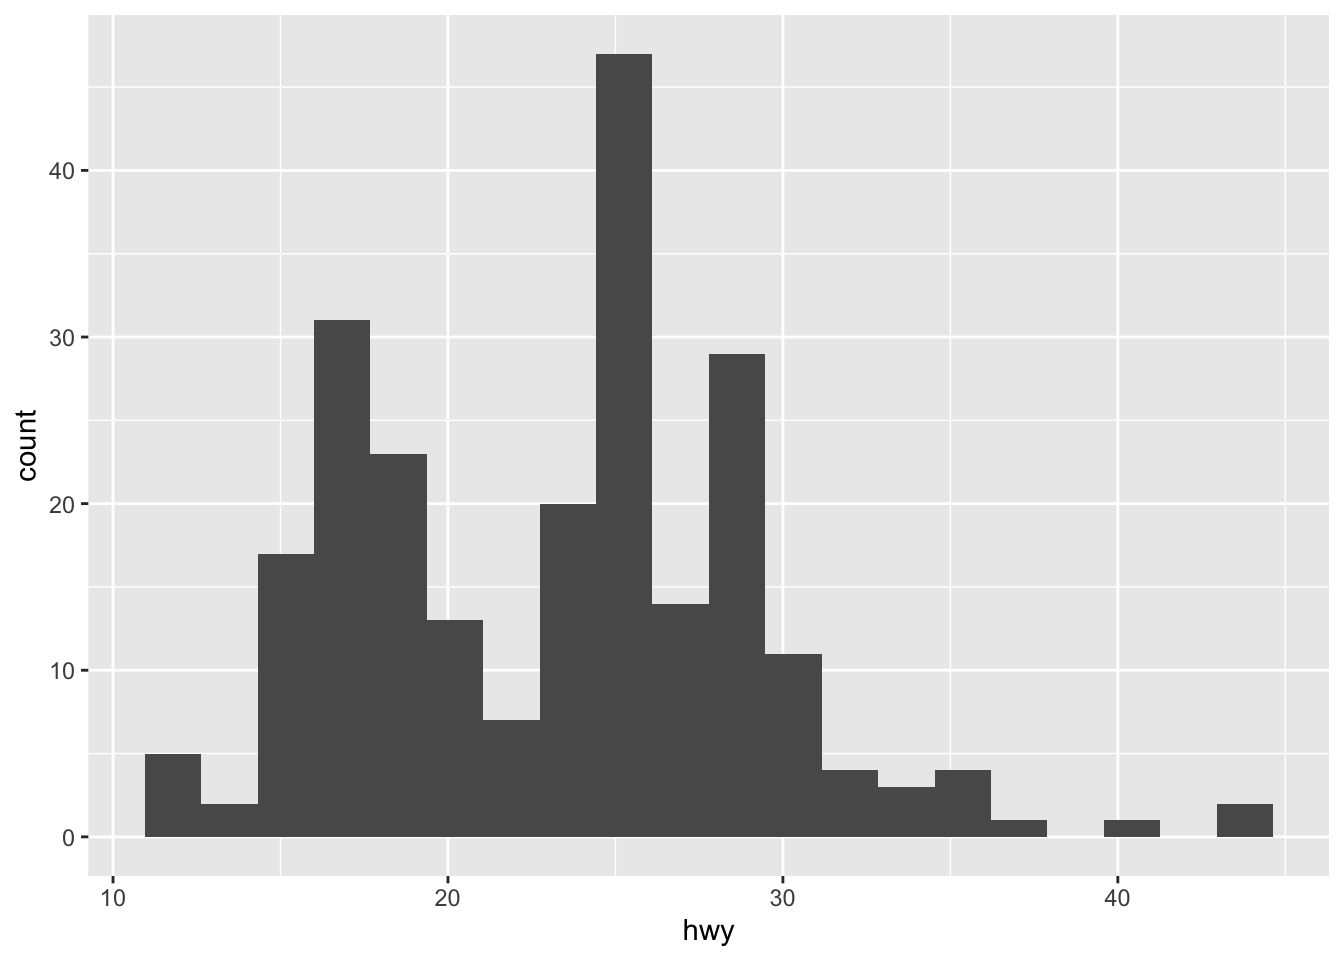
\includegraphics{_main_files/figure-latex/unnamed-chunk-14-1.pdf}

\hypertarget{mmrf-commpass-datasets}{%
\chapter{MMRF CoMMpass datasets}\label{mmrf-commpass-datasets}}

This codebook will rely on data from the MMRF CoMMpass data. Register as a researcher and download the following data from release IA21 \href{https://research.themmrf.org/population/\#/ds/6262ea84d1211200016ce44c/downloads}{https://research.themmrf.org/} in a directory named \texttt{MMRF\_IA21}.

\begin{verbatim}
CoMMpass_IA21_FlatFile_Dictionaries.tar.gz # decompress this folder
CoMMpass_IA21_FlatFiles.tar.gz # decompress
\end{verbatim}

\hypertarget{explore-mmrf-commpass-clinical-variables}{%
\section{Explore MMRF CoMMpass clinical variables}\label{explore-mmrf-commpass-clinical-variables}}

\begin{Shaded}
\begin{Highlighting}[]
\FunctionTok{library}\NormalTok{(tidyverse)}
\end{Highlighting}
\end{Shaded}

\begin{verbatim}
## Warning: package 'tidyverse' was built under R version 4.1.2
\end{verbatim}

\begin{verbatim}
## Warning: package 'tibble' was built under R version 4.1.2
\end{verbatim}

\begin{verbatim}
## Warning: package 'tidyr' was built under R version 4.1.2
\end{verbatim}

\begin{verbatim}
## Warning: package 'readr' was built under R version 4.1.2
\end{verbatim}

\begin{verbatim}
## Warning: package 'purrr' was built under R version 4.1.2
\end{verbatim}

\begin{verbatim}
## Warning: package 'dplyr' was built under R version 4.1.2
\end{verbatim}

\begin{verbatim}
## Warning: package 'stringr' was built under R version 4.1.2
\end{verbatim}

\begin{verbatim}
## Warning: package 'forcats' was built under R version 4.1.2
\end{verbatim}

\begin{verbatim}
## Warning: package 'lubridate' was built under R version 4.1.2
\end{verbatim}

\begin{verbatim}
## -- Attaching core tidyverse packages ------------------------ tidyverse 2.0.0 --
## v dplyr     1.1.2     v readr     2.1.4
## v forcats   1.0.0     v stringr   1.5.0
## v lubridate 1.9.2     v tibble    3.2.1
## v purrr     1.0.1     v tidyr     1.3.0
## -- Conflicts ------------------------------------------ tidyverse_conflicts() --
## x dplyr::filter() masks stats::filter()
## x dplyr::lag()    masks stats::lag()
## i Use the conflicted package (<http://conflicted.r-lib.org/>) to force all conflicts to become errors
\end{verbatim}

  \bibliography{book.bib,packages.bib}

\end{document}
